\section{The Mezuro Project}
\label{sec:mezuro}

The Mezuro project~\cite{mezuro2012} aims to be an interface which allows, in a
flexible way, the extraction, analysis and interpretation of static source code
metrics. Licensed under the Affero General Public License version 3 (AGPLv3),
it allows users define the metrics they want to employ on the analysis, keeping
track and providing graphical visualization of the evolution of the selected
set of metrics. From here the set of selected metrics together with the
interpretations for each value  will be referenced just as ``configuration''.
Its main academical goals are: to get close to a consensus on which
configurations should be employed on the analysis of different kinds of source
code written in different programming languages and to search which
interpretation should be given to each value obtained for the
configuration~\cite{meirelles2013}.

\subsection{Early design}
\label{subsec:early-design}

Initially, we developed a desktop prototype for the QualiPSo project called
Kalibro \cite{de2013kalibro}, written in Java which had many of the features we
wanted for source code analysis. At that time, Kalibro already supported the
selection and composition of metrics to be employed on the analysis and allowed
users to define their own interpretation for the results of each metric
calculation.  With a created configuration, Kalibro only needed an URL for the
source code to start the analysis. The URL could be the path for the source
code, compressed in a ZIP or TARBALL file, on the user's computer or the link
for the repository where the source code was stored. The source code managers
supported included GIT, Subversion, CVS, Mercurial and Bazaar. Finally, the
source code could be written in either Java, C, or C++, according to Analizo
supported programming languages.

\begin{figure}[htb]
  \centering
  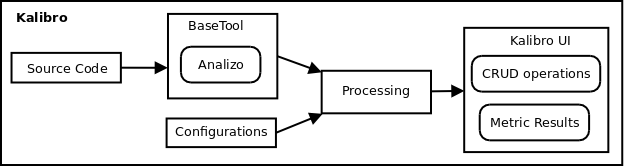
\includegraphics[width=\textwidth]{images/kalibro-initial-arch.png}
  \caption{Architecture of the initial implementation.}
  \label{fig:kalibro-initial-arch}
\end{figure}

\textbf{Figure \ref{fig:kalibro-initial-arch}} represents the initial
implementation with Kalibro components well defined. In short, it was
integrated to its first basetool, working as a front-end to Analizo. Despite
Kalibro being capable to successfully analyze source codes, we could not get
close to the consensus we aimed for. The main obstacle was that, with a desktop
application, it was not possible to incite the discussion on the configurations
employed among developers nor the comparison of results between projects. That
was the main reason that motivated the move from a desktop application to a
service-based implementation.

\subsection{Service-based implementation}
\label{subsec:service-based-implementation}

The first service-based implementation was designed to working on a BI
environment called Spago4Q~\footnote{\url{spago4q.org}} in the QualiSPo project
context. Kalibro just provides a set of metric results to be extracted and
reported by Spago4Q.
%
After that, Kalibro evolved to a monolithic web service that performed all the
database and analysis operations. It was integrated to a plugin of the
Noosfero\footnote{\url{noosfero.org}} social networking platform. At that time,
the plugin and all project was named Mezuro.


The back-end was described in WSDL and communicated with the front-end using
SOAP messages.  It was still written in Java for it was an extension of
Kalibro. As for the front-end, we wanted that our users were able to discuss
and compare their configuration and results. Thus, a social network seemed a
good way to achieve that. We did not want to implement a social network from
scratch, though.  Noosfero was a good choice for its robust plugin support and
for being open source. Mezuro plugin was written in Ruby, using the Ruby on
Rails framework. \textbf{Figure \ref{fig:mezuro-noosfero-arch}} represents the
state diagram for the service-based implementation. This is a simplified
diagram for it omits some entities of our system as the reading groups, which
abstract the interpretations given for the metrics and are part of the
configurations.

\begin{figure}[htb]
  \centering
  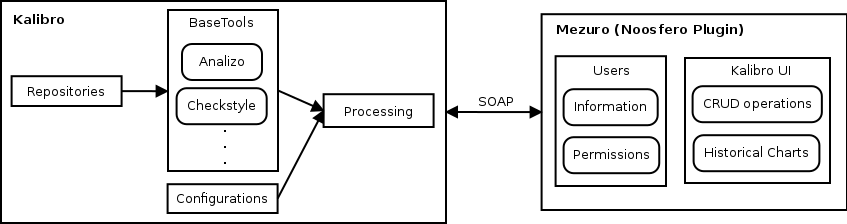
\includegraphics[width=\textwidth]{images/mezuro-noosfero-arch.png}
  \caption{Architecture of the service-based implementation.}
  \label{fig:mezuro-noosfero-arch}
\end{figure}

With this new implementation, Mezuro allowed users to create their own
configurations of metrics and respective interpretations. They could register
the URL for their repositories on GIT or Subversion. Most importantly, they
could view and compare their results with the repositories of other users. That
data could be used in order to extend the research on source code metrics and
software quality within free software projects. Mezuro supports source codes
written on Java, C, and C++, also with CheckStyle as Java metric collector.

The main advantage of this implementation was to bring the code analysis tools
to the web in a way that multiple users could produce their own configurations
as well as view and share historical results from their analysed projects.
However, on the front-end, the major issue was that the technologies used were
outdated making it difficult for maintenance and development. Also, Noosfero
had features that we did not need for our social network such as the support
for communities and events. For the web service being monolithic, minor changes
on the source code implied a full deploy of the system. In short, it was hard to
understand and modify it. That slowed down our productivity. Still, the main
disadvantage was the scalability.

We started worrying about scalability when we were about to release Mezuro to
the community. We wanted to assess if Kalibro web service could keep its
performance when changes on the workload occurred. For the tests, we used the
Scalability Explorer\cite{moura2013automated} framework. We calculated three
metrics available on the framework: speed-up, degradation, and aggregate
performance comparison\cite{li2012catalogue}. We found that our most important
feature, the process repository operation, was not scalable. Worse, for big
workloads Kalibro simply stopped working without errors. Further investigation
showed us that this sudden interruption happened due to a deadlock.

The problem was on the static thread pool created by Kalibro web service. By
default, Kalibro created a static thread pool with a variable number of
threads, depending on the machine it was running on. The threads were kept
idle, waiting for some operation to awake them. Each source code analysis
required four threads to complete because parts of that operation were made in
parallel. The operation awoke the threads on demand, that it, only when it was
going to use them. Therefore, if a great number of requests for the process
repository operation reached the service simultaneously, those operations would
start but would not be able to finish because of a lack of threads available.

With difficulties for modifying the code to support a dynamic thread pool, our
solution was to rewrite the service. Thus, we could solve the deadlock issue
and improve the service architecture.

\subsection{Cloud-based implementation}
\label{subsec:cloud-based-implementation}

With the rewritten code, Mezuro project was split into three different
services: Prezento, Kalibro Processor, and Kalibro Configurations. The user
interface, code analyzer, and configuration manager, respectively. We designed
Kalibro onto two separated services with the intention of leaving each of them
with less responsibilities, making them easier to maintain and to extend.
Furthermore, it allows other developers to reuse them flexibly. For example, if
someone desires to implement its own source code analyzer, that developer can
utilize Kalibro Configurations for managing metrics and their interpretations.
Those services communicate through HTTP requests encapsulated onto a fourth
piece of software called Kalibro Client.  All of them are written in Ruby with
the support of the Ruby on Rails framework. The reason for switching WSDL and
SOAP for RESTful APIs was its significantly simpler implementation.

All this work is based on the micro-service architecture
\cite{namiot2014micro}. With this new distributed architecture, the platform has
more flexibility to scale into the cloud. It as well demands less knowledge
from developers about the existing code, since they do not need to know all the
services but just the one which relates to the feature being implemented and
its API. Other advantages are that each service can be written in different
programming languages and, for each service runs its own processes, they can be
deployed independently. That also enhances fault tolerance.

Furthermore, better scalability was achieved with the help of the ActiveJob
gem\footnote{\url{github.com/rails/rails/tree/master/activejob}}.  ActiveJob
creates a queue of operations to be executed some time in the future by a
number of workers defined by the user. In our case, we have created a queue for
the source code analysis operation with 16 workers. That way, we are able to
keep Prezento running while all source code analysis required runs on
background. However, the main disadvantages of the micro-services architecture
are that it is more complex and, if the API of one of the services change, the
others that use it must adapt to keep the communication working.

\textbf{Figure \ref{fig:mezuro-cloud-arch}} refers to the state diagram for the
cloud-based implementation. Again, there are implicit details we omitted to
keep the simplicity as the Kalibro Client gem that encapsulates the exchanged
HTTP messages among the services.

\begin{figure}[htb]
  \centering
  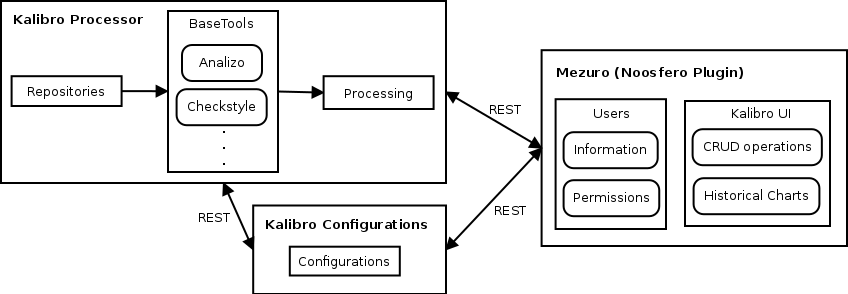
\includegraphics[width=\textwidth]{images/mezuro-cloud-arch.png}
  \caption{Architecture of the cloud-based implementation.}
  \label{fig:mezuro-cloud-arch}
\end{figure}

This final step on the evolution of the Mezuro project brings it to the new era
of cloud computing with scalability, distributed processing, and fault
tolerance through the described division into smaller services. That
modularization enables the system to scale each of its components on demand. As
well it provides to developers the flexibility necessary for expansions such as
adding support for collecting source code metrics from other programming
languages, which is the current effort of our team.

As result of the described evolution through time here are summarized the main
features of Mezuro:

\begin{itemize}

  \item Latest standards on web development (through Boilerplate and
	TwitterBootstrap frameworks) brings a clean interface, easy to use, and familiar
	to others found by users on the web;

  \item Multi-user environment with permission management which allows the
	collaboration and spreading of standards;

  \item Historical data about the evolution of metric values through time;

  \item Multi-language support for analysis;

  \item Configurable set of metrics and interpretations which enables it to
	suit better to the variety of projects in the world;

  \item Distributed services with specific responsibilities which makes them
	easier to extend and install on cloud infrastructures.

\end{itemize}
